\section{Martingales}

  Let us first start with the discrete-time martingale for simplicity. In introductory courses, a martingale might be defined as a \hyperref[def:stochastic-process]{stochastic process} satisfying 

    \begin{equation}
      X_n = \mathbb{E}[X_{n+1} \mid X_0, \ldots, X_n]
    \end{equation}

  for all $n$, which models a "fair game." They also may construct the \hyperref[prob-def:random-variable]{random variables} $\{X_n\}$ first and then define the \hyperref[def:filtration]{filtration} as the sequence of $\sigma$-algebras $\sigma(X_1, \ldots, X_n)$. In here, we will construct the filtration $\{\mathcal{F}_n\}$ first and then define the random variables to be adapted to the filtration if $X_n$ is $\mathcal{F}_n$-measurable for each $n \in \mathbb{N}$. 

  \begin{definition}[Discrete-Time Martingale]
    \label{def:discrete-time-martingale}
    Given a \hyperref[prob-def:probability-space]{probability space} $(\Omega, \mathcal{F}, \mathbb{P})$, let $\mathbb{F} = \{\mathcal{F}_n\}_{n \in \mathbb{N}}$ be a \hyperref[def:filtration]{filtration} (an increasing sequence of $\sigma$-algebras). A sequence $\{X_n\}$ is said to be \textbf{adapted} to $\{\mathcal{F}_n\}$ if $X_n$ is $\mathcal{F}_n$-measurable for all $n$. If the \hyperref[def:stochastic-process]{stochastic process} $\{X_n\}_{n \in \mathbb{N}}$ is a sequence with 

    \begin{enumerate}
      \item $\mathbb{E}[X_n] < \infty$ for all $n$, 
      \item $X_n$ is adapted to $\mathcal{F}_n$, 
      \item $\mathbb{E}[X_{n+1} \mid X_1, \ldots, X_n] = \mathbb{E}[X_{n+1} \mid \mathcal{F}_n] = X_n$ for all $n$, 
    \end{enumerate}

    then $\{X_n\}$ is a \textbf{\hyperref[def:martingale]{martingale}}. If $\mathbb{E}[X_{n+1} \mid \mathcal{F}_n] \leq X_n$ or $\mathbb{E}[X_{n+1} \mid \mathcal{F}_n] \geq X_n$, the $\{X_n\}$ is said to be a \textbf{supermartingale} or \textbf{submartingale}, respectively. 
  \end{definition}

  A \hyperref[def:martingale]{martingale} just represents a sequence of \hyperref[prob-def:random-variable]{random variables} that get finer and finer as the $\sigma$-algebra increases. While they do get finer and finer, they do not change the "average" of the function. For example, consider the \hyperref[def:filtration]{filtration} generated by finer subsets of the unit interval $\Omega = (0, 1]$. We have 

  \begin{enumerate}
    \item $\mathcal{F}_0 = \{\emptyset, \Omega\}$ 
    \item $\mathcal{F}_1 = \sigma( (0, 0.5], (0.5, 1])$ 
    \item $\mathcal{F}_2 = \sigma( (0, 0.25], (0.25, 0.5], (0.5, 0.75], (0.75, 1] )$
  \end{enumerate}

  Then, we would have 

  \begin{center}
    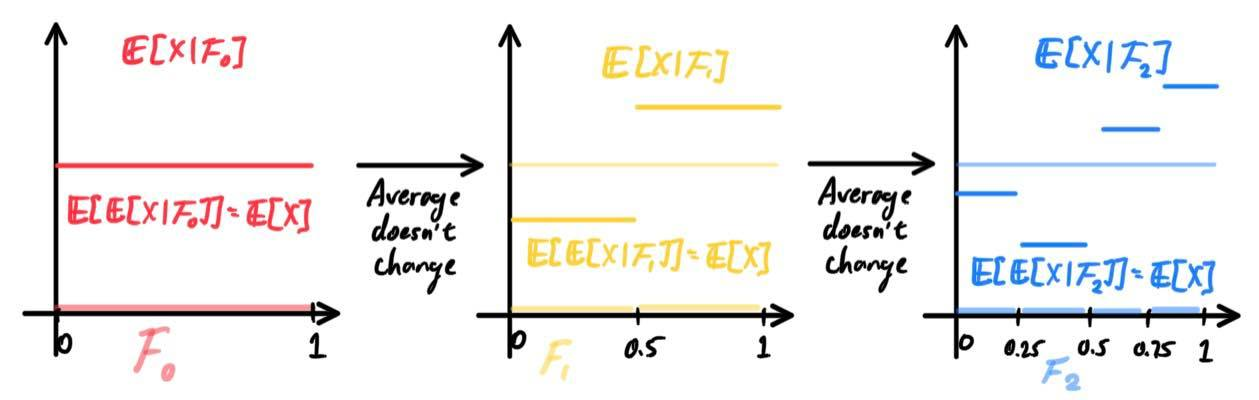
\includegraphics[scale=0.3]{img/martingale_increments.jpg}
  \end{center}
  
  A supermartingale (and submartingale) just means that as we make the function finer and finer, its mean goes down (or up). 


  Martingales are used to model lots of random walk events. In the following three examples, let $\xi_1, \xi_2, \ldots$ be iid, and let $S_n = S_0 + \xi_1 + \ldots + \xi_n$., where $S_0$ is a constant. Let $\mathcal{F}_n = \sigma(\xi_1, \ldots, \xi_n)$ for $n \geq 1$ and let $\mathcal{F}_0 = \{\emptyset, \Omega\}$. 

  \begin{example}[Linear Martingale]
    \label{ex:linear-martingale}
    Let $\mu = \mathbb{E}[\xi_i] = 0$. Then, $\{S_n\}$ is a martingale with respect to $\mathcal{F}_n$. We show the three requirements: 
    \begin{enumerate}
      \item $\mathbb{E}[S_n] = \mathbb{E}[S_0] + \mathbb{E}[\xi_1] + \ldots + \mathbb{E}[\xi_n] = S_0 < \infty$. 
      
      \item By definition, we know that $\xi_i$ is $\sigma(\xi)$-measurable for all $i \in [n]$, so $\xi_i$ is $\mathcal{F}_n = \sigma(\xi_1, \ldots, \xi_n)$-measurable. Since the set of $\mathcal{F}_n$-measurable functions has a \hyperref[lin-def:vector-space]{vector space} structure, $S_n$ is also $\mathcal{F}_n$-measurable. 
      
      \item We can simply solve 

        \begin{equation}
          \mathbb{E}[S_{n+1} \mid \mathcal{F}_n] = \mathbb{E}[S_n \mid \mathcal{F}_n] + \mathbb{E}[\xi_{n+1} \mid \mathcal{F}_n] = X_n + \mathbb{E}[\xi_{n+1}] = X_n
        \end{equation}

      where the first equality follows from linearity. For the second equality, note that $S_n$ is $\mathcal{F}_n$-measurable from above, and so the best $\mathcal{F}_n$-measurable approximation of $X$ is $X$ itself (i.e. we have complete information). We know that $\xi_{n+1}$ is independent of the $\xi_i$'s, and so by definition their $\sigma$-algebras are independent. This implies that $\sigma(\xi_{n+1})$ and $\mathcal{F}_n = \sigma(\xi_1, \ldots, \xi_n)$ are independent, and so due to irrelevant information, $\mathbb{E}[\xi_{n+1} \mid \mathcal{F}_n] = \mathbb{E}[\xi_{n+1}]$. 
    \end{enumerate}
    If $\mu \leq 0$ or $\mu \geq 0$, then the computation above shows that $\mathbb{E}[S_{n+1} \mid \mathcal{F}_n] \leq 0$ or $\mathbb{E}[S_{n+1} \mid \mathcal{F}_n] \geq 0$, making it a supermartingale or submartingale, respectively. 
  \end{example}

  Given a supermartingale or submartingale, we can change it to be a \hyperref[def:martingale]{martingale}. 

  \begin{example}[Centred Random Walk as a Martingale]
    \label{ex:centred-random-walk-as-a-martingale}
  Given that $\mu = \mathbb{E}[\xi_i] \neq 0$, then $\{S_n - n\mu\}$ is a martingale with respect to $\mathcal{F}_n$. We can see this because

  \begin{align*}
    \mathbb{E}[S_{n+1} - (n + 1)\mu \mid \mathcal{F}_n] & = \mathbb{E}[S_n - n \mu \mid \mathcal{F}_n] + \mathbb{E}[\xi_{n+1} - \mu \mid \mathcal{F}_n] \\
    & = S_n - n \mu + \mathbb{E}[\xi_{n+1}] - \mu \\
    & = S_n - n
  \end{align*}
  \end{example}

  \begin{example}[Quadratic Martingale]
    \label{ex:quadratic-martingale}
  Say $\mu = \mathbb{E}[\xi_i] = 0$ and $\sigma^2 = \mathrm{Var}(\xi_i) < \infty$. Then, $\{S_n^2 - n \sigma^2\}$ is a martingale. 

  \begin{align*}
    \mathbb{E}[S_{n+1}^2 - (n + 1) \sigma^2 \mid \mathcal{F}_n] & = \mathbb{E}[ (S_n + \xi_{n+1})^2 - (n _ 1) \sigma^2 \mid \mathcal{F}_n] \\
    & = \mathbb{E}[S^2 - n \sigma^2 \mid \mathcal{F}_n ] + \mathbb{E}[ 2 S_n \xi_{n+1} + \xi_{n+1}^2 - \sigma^2 \mid \mathcal{F}_n] \\
    & = \mathbb{E}[S^2 - n \sigma^2 \mid \mathcal{F}_n ] + 2 \mathbb{E}[ S_n \xi_{n+1} \mid \mathcal{F}_n ] + \mathbb{E}[\xi_{n+1}^2] - \sigma^2  \\
    & = \mathbb{E}[S^2 - n \sigma^2 \mid \mathcal{F}_n ]
  \end{align*}

  where we have used the fact that due to independence of $\xi_{n+1}$ with $\mathcal{F}_n$, we have $\mathbb{E}[S_n \xi_{n+1} \mid \mathcal{F}_n] = \mathbb{E}[S_n \mathbb{E}[ \xi_{n+1} \mid \mathcal{F}_n]] = \mathbb{E}[S_n \cdot 0] = 0$. 
  \end{example}

  This following result shows that \hyperref[def:martingale]{martingales} with bounded increments either converge or oscillate between $+\infty$ and $-\infty$. 

  \begin{theorem}[Martingale Convergence under Bounded Increments]
    \label{thm:martingale-convergence-under-bounded-increments}
    Let $\{X_n\}_{n \in \mathbb{N}}$ be a \hyperref[def:martingale]{martingale} with $|X_{n+1} - X_n| \leq M < \infty$. Let 

    \begin{align*}
      C & = \{\lim_{n \rightarrow \infty} X_n \text{ exists and is finite}\} \\
      D & = \{\lim_{n \rightarrow \infty} \sup X_n = +\infty \text{ and } \lim_{n \rightarrow \infty} \inf X_n = -\infty\}
    \end{align*}

    Then $\mathbb{P}(C \cup D) = 1$. 
  \end{theorem}

  Note that as you get more and more information, your $\sigma$-algebra can "grow" and get closer to something that models complete information. This means that given some $\sigma$-algebra $\mathcal{F}$ that models complete information, we can take a sequence of nondecreasing sub-$\sigma$-algebras of $\mathcal{F}$ 
  \begin{equation}
    \mathcal{F}_1 \subset \mathcal{F}_2 \subset \ldots \subset \mathcal{F}_i \subset \ldots
  \end{equation}
  such that $\mathcal{F}_i \subset \mathcal{F}$, which models our increasing knowledge of the experiment. 



  \begin{example}[Filtration of 3 Coin Tosses]
    \label{ex:filtration-of-3-coin-tosses}
    Let us describe a concrete example of a 3-coin toss filtration. The \hyperref[prob-def:probability-space]{probability space} is 
    \begin{equation}
      \Omega = \{000, 001, 010, 011, 100, 101, 110, 111\}
    \end{equation}
    which has $8$ outcomes so a complete $\sigma$-algebra would consist of $2^8 = 256$ outcomes. 
    \begin{enumerate}
      \item Before the experiment, we have no information at all, so 
      \begin{equation}
        \mathcal{F}_0 = \{\emptyset, \Omega\}
      \end{equation}
      which has $2^{2^0} = 2$ elements. 
      
      \item After the first coin toss, we would have information on what the first flip landed on (whether it was of form $( 0, \ast, \ast)$ or $(1, \ast, \ast)$), so we have a $\sigma$-algebra generated by these two events 
      \begin{align*}
        \mathcal{F}_1 & = \sigma(\{( 0, \ast, \ast)\}, \{(1, \ast, \ast)\}) \\
        & = \sigma(\{000, 001, 010, 011\}, \{100, 101, 110, 111\}) \\
        & = \{\emptyset, \{000, 001, 010, 011\}, \{100, 101, 110, 111\}, \Omega\}
      \end{align*}
      which has $2^{2^1} = 4$ elements. 
      
      \item After the second coin toss, we would have information on what the first two flips landed on (whether it was of form $( 0, 0, \ast)$, $( 0, 1, \ast)$, $(1, 0, \ast)$, $(1, 1, \ast)$), so we have a $\sigma$-algebra generated by these 4 events 
      \begin{align}
        \mathcal{F}_2 & = \sigma(\{( 0, 0, \ast)\}, \{( 0, 1, \ast)\}, \{(1, 0, \ast)\}, \{(1, 1, \ast)\}) \\
        & = \sigma(\{000, 001\}, \{010, 011\}, \{100, 101\}, \{110, 111\}) \\
        & = \{\emptyset, \{000, 001\}, \{010, 011\}, \{100, 101\}, \{110, 111\}, \\
        & \;\;\;\;\;\; \{000, 001, 010, 011\}, \{000, 001, 100, 101\}, \{000, 001, 110, 111\}, \\
        & \;\;\;\;\;\; \{010, 011, 100, 101\}, \{010, 011, 110, 111\}, \{100, 101, 110, 111\}, \\ 
        & \;\;\;\;\;\; \{000, 001, 010, 011, 100, 101\}, \{000, 001, 010, 011, 110, 111\}, \\
        & \;\;\;\;\;\; \{000, 001, 110, 101, 110, 111\}, \{010, 011, 110, 101, 110, 111\},  \Omega\}
      \end{align}
      which has $2^{2^2} = 16$ elements. 
      
      \item After the third coin toss, we would have information on what the first three flips landed on (all 8 possibilities in $\Omega$), so we have a $\sigma$-algebra generated by these 8 events 
      \begin{align}
        \mathcal{F}_3 & = \sigma(\{000\}, \{001\}, \{010\}, \{011\}, \{100\}, \{101\}, \{110\}, \{111\})
      \end{align}
      This is too big to write down explicitly, but it has $2^{2^3} = 256$ elements. 
    \end{enumerate}
  \end{example}


	Remember that for a \hyperref[prob-def:random-variable]{random variable} $X$ and $\sigma$-algebras $\mathscr{F}_1, \mathscr{F}_2$ s.t. $\mathscr{F}_1 \subset \mathscr{F}_2$, by the tower property, 
	\begin{equation}
		\mathbb{E}[ \mathbb{E}[X \mid \mathscr{F}_2] \mid \mathscr{F}_1] = \mathbb{E}[X \mid \mathscr{F}_1] 
	\end{equation}

	If we exchange the two, the smaller one wins. but for arbitrary $\sigma$-algebras, equality does not hold.\footnote{No direct connection to \hyperref[mt-thm:fubinis-theorem]{Fubini's theorem}.}
	\begin{equation}
		\mathbb{E}[ \mathbb{E}[X \mid \mathscr{F}_2] \mid \mathscr{F}_1] \neq \mathbb{E}[ \mathbb{E}[X \mid \mathscr{F}_1] \mid \mathscr{F}_2]
	\end{equation}

	It is useful to consider when $\mathscr{F}_2 \not\subset \mathscr{F}_1$ and $\mathscr{F}_1 \not\subset \mathscr{F}_2$. 

	\begin{example}[Filtrations on a Three-Point Space]
	  \label{ex:filtrations-on-a-three-point-space}
		The prototypical example is $\Omega = \{a, b, c\}$ with $\mathbb{P}(\{a\}) = \mathbb{P}(\{b\}) = \mathbb{P}(\{c\}) = \frac{1}{3}$. Then, $X(a) = 1, X(b) = 2, X(c) = 3$. Consider the following $\sigma$-algebras: 
		\begin{enumerate}
			\item $\mathscr{F}_1$ generated by $\{a, b\}, \{c\}$. 
			\item $\mathscr{F}_2$ generated by $\{a\}, \{b, c\}$. 
		\end{enumerate}
		Then, 
		\begin{align}
			\mathbb{E}[X \mid \mathscr{F}_1](\omega) & = \begin{cases} 
				1.5 & \text{ if } \omega \in \{a, b\} \\ 
				3 & \text{ if } \omega \in \{c\} 
			\end{cases} \implies \mathbb{E}[ \mathbb{E}[X \mid \mathscr{F}_1] \mid \mathscr{F}_2] = 
			\begin{cases} 
				1.5 & \text{ if } \omega \in \{a\} \\ 
				2.75 & \text{ if } \omega \in \{b, c\} 
			\end{cases} \\ 
			\mathbb{E}[X \mid \mathscr{F}_2](\omega) & = \begin{cases} 
				1 & \text{ if } \omega \in \{a\} \\ 
				2.5 & \text{ if } \omega \in \{b, c\} 
			\end{cases} \implies \mathbb{E}[ \mathbb{E}[X \mid \mathscr{F}_2] \mid \mathscr{F}_1] = 
			\begin{cases} 
				1.75 & \text{ if } \omega \in \{a, b\} \\ 
				2.5 & \text{ if } \omega \in \{c\} 
			\end{cases}
		\end{align}
	\end{example}

	

	\begin{definition}[Martingale]
	  \label{def:martingale}
	  If $X_n$ further satisfies 
		\begin{enumerate}
			\item $\mathbb{E}[|X_n|] < +\infty$ (so that we don't run into any problems in cord exp)
			\item $\mathbb{E}[X_n \mid \mathscr{F}_{n-1}] = X_{n-1}$. 
		\end{enumerate}
		Then $(X_n)$ is called a \textbf{martingale}. If instead of (2), we have 
		\begin{enumerate}
		  \item $\mathbb{E}[X_n \mid \mathscr{F}_{n-1}] \leq X_{n-1}$, then $(X_n)$ is a \textbf{supermartingale}. 
		  \item $\mathbb{E}[X_n \mid \mathscr{F}_{n-1}] \geq X_{n-1}$, then $(X_n)$ is a \textbf{submartingale}. 
		\end{enumerate}
	\end{definition}

	\begin{example}[Random Walk]
	  \label{ex:random-walk}
	  Let $Y_1, \ldots$ be iid \hyperref[prob-def:random-variable]{random variables} and define 
		\begin{equation}
			S_n = S_0 + \sum_{i=1}^n Y_i
		\end{equation}
		where $S_0$ is a constant. To specify a \hyperref[def:filtration]{filtration}, a canonical way of constructing it is to just let it be generated by the random variables. So, 
		\begin{equation}
			\mathscr{F}_0 = \{\empty,  \Omega\}, \qquad \mathscr{F}_n = \sigma(Y_1, \ldots, Y_n)
		\end{equation}
		For (1) to hold, just assume $\mathbb{E}[|Y_i|] < +\infty \implies \mathbb{E}[|S_n|] < +\infty$ by triangle inequality. So, by our construction, we get 
		\begin{equation}
			\mathbb{E}[S_n \mid \mathscr{F}_{n-1}] = \underbrace{S_0 + \sum_{i=1}^{n-1} Y_i}_{= S_{n-1}} + \underbrace{\mathbb{E}[Y_n \mid \mathscr{F}_{n-1}]}_{= \mathbb{E}[Y_n]} 
		\end{equation}
		where $\mathbb{E}[Y_n \mid \mathscr{F}_{n-1}] = \mathbb{E}[Y_n]$ since $Y_n$ is independent of $\mathscr{F}_{n-1}$. So, 
		\begin{enumerate}
			\item if $\mathbb{E}[Y_n] = 0$, $S_n$ is a \hyperref[def:martingale]{martingale}. 
			\item if $\mathbb{E}[Y_n] > 0$, $S_n$ is a submartingale. 
			\item if $\mathbb{E}[Y_n] < 0$, $S_n$ is a supermartingale. 
		\end{enumerate}
	\end{example}

	\begin{example}[Products of Nonnegative Random Variables]
	  \label{ex:products-of-nonnegative-random-variables}
	  Now let 
		\begin{equation}
			M_n = \prod_{i=1}^n Y_i, \qquad Y_i \geq 0
		\end{equation}
		and assume $\mathbb{E}[Y_i]^2 < +\infty$. Then, by \hyperref[prob-thm:cauchy-schwarz]{Cauchy-Schwarz}, $\mathbb{E}[|M_n|] < +\infty$. Then, 
		\begin{equation}
			\mathbb{E}[M_n \mid \mathscr{F}_{n-1}] = \bigg( \prod_{i=1}^n Y_i \bigg) \mathbb{E}[Y_n] = M_{n-1} \mathbb{E}[Y_n]
		\end{equation}
		So, 
		\begin{enumerate}
			\item if $\mathbb{E}[Y_n] = 1$, $S_n$ is a \hyperref[def:martingale]{martingale}. 
			\item if $\mathbb{E}[Y_n] > 1$, $S_n$ is a submartingale. 
			\item if $\mathbb{E}[Y_n] < 1$, $S_n$ is a supermartingale. 
		\end{enumerate}
	\end{example}

	Now for some abstract properties of \hyperref[def:martingale]{martingales}. 

	\begin{lemma}[Supermartingale Inequality over Several Steps]
	  \label{thm:supermartingale-inequality-over-several-steps}
 
		If $X_n$ is a supermartingale, then for all $n > m$, $\mathbb{E}[X_n \mid \mathscr{F}_m] \leq X_m$.
	\end{lemma}
	\begin{proof}
	  Induct on $n$ and tower property. 
		\begin{align}
			\mathbb{E}[X_n \mid \mathscr{F}_m] & = \mathbb{E}[\mathbb{E}[X_n \mid \mathscr{F}_{n-1}] \mid \mathscr{F}_m ] && \tag{Tower Property} \\ 
																				 & \leq \mathbb{E}[X_{n-1} \mid \mathscr{F}_m ] && \tag{By Definition} \\ 
																				 & \leq X_m && \tag{Inductive Hypothesis}
		\end{align}
	\end{proof}

	\begin{corollary}[Multi-Step Submartingale and Martingale Identities]
	  \label{thm:multi-step-submartingale-and-martingale}
	  Let $X_n$ be adapted to the filtration $\mathscr{F}_n$. Then the following hold. 
		\begin{enumerate}
			\item If $X_n$ is a submartingale, then for all $n > m$, $\mathbb{E}[X_n \mid \mathscr{F}_m] \geq X_m$. 
			\item If $X_n$ is a  \hyperref[def:martingale]{martingale}, then for all $n > m$, $\mathbb{E}[X_n \mid \mathscr{F}_m] = X_m$. 
		\end{enumerate}
	\end{corollary}
	\begin{proof}
		We use the common ``symmetry trick.''
		\begin{enumerate}
		  \item $-X_n$ is a supermartingale and use the lemma. 
			\item $X_n$ is both a supermartingale and submartingale. 
		\end{enumerate}
	\end{proof}

	\begin{definition}[Predictable Sequence]
	  \label{def:predictable-sequence}
		For a \hyperref[def:filtration]{filtration} $(\mathscr{F}_n)_{n=0}^\infty$, a sequence of \hyperref[prob-def:random-variable]{random variables} $(H_n)_{n=1}^\infty$ is a \textbf{predictable sequence} if $H_n$ is measurable with respect to $\mathscr{F}_{n-1}$. 
	\end{definition}

	It is immediate that \hyperref[def:predictable-sequence]{predictable sequences} are adapted, since the $\sigma$-algebras are increasing in a \hyperref[def:filtration]{filtration}, i.e. $H_n$ is $\mathscr{F}_{n-1}$-measurable which implies $H_n$ is $\mathscr{F}_n$ measurable. Adapated sequences are not necessarily predictable. 

	\begin{example}[Gambling]
	  \label{ex:gambling}
	  At each round $r$, you bet \$x. With probability $p$, you win an additional \$x and with probability $1-p$, you lose \$x. Let 
		\begin{enumerate}
		  \item $X_n = $ not winning after $n$ rounds, if you bet \$1 each time. 
			\item $H_n = $ amount of money you bet in round $n+1$. So, makes sense to be $\mathscr{F}_{n+1}$-measurable. So, this is an example of a \hyperref[def:predictable-sequence]{predictable sequence}. 
			\item Now, our net earnings after $n$ rounds of the game is 
				\begin{equation}
					(H \cdot X)_n = \sum_{m=1}^n H_m (X_m - X_{m-1})
				\end{equation}
				where $X_m - X_{m-1} \in \{\pm 1\}$. 
		\end{enumerate}
		Now the strategy might be to double down if you lose, and keep betting \$1 if you win, so 
		\begin{equation}
			H_n = \begin{cases} 
				2 H_{n-1} & \text{ if } X_{n-1} - X_{n-2} = -1 \\ 
				1 & \text{ if } X_{n-1} - X_{n-2} = \pm 1
			\end{cases} 
		\end{equation}
		This betting strategy is called a \hyperref[def:martingale]{martingale}. Remember that if we had infinite money, we will always win. More generally, if $(H \cdot X)_n$ is a submartingale, then $\mathbb{E}[(H \cdot X)_n] \geq 0$. So, we should consider cases which leads to $(H \cdot X)_n$ being a submartingale. 
	\end{example}

	\begin{theorem}[Discrete Stochastic Integral of a Supermartingale]
	  \label{thm:discrete-stochastic-integral-of-a}
		Let $X_n$, $n \geq 0$ be a supermartingale. If $H_n \geq 0$ is predictable and each $H_n$ is bounded (pointwise), then $(H \cdot X)_n$ is a super-martingale. 
	\end{theorem}
	\begin{proof}
	  We have 
		\begin{align}
			\mathbb{E}[(H \cdot X)_{n+1} \mid \mathscr{F}_n] & = (H \cdot X)_n + \mathbb{E}[H_{n+1} (X_{n+1} - X_n) \mid \mathscr{F}_n ] \\ 
																											 & = (H \cdot X)_n + H_{n+1} \mathbb{E}[\underbrace{X_{n+1} - X_n}_{\leq 0} \mid \mathscr{F}_n ] \\ &
																											& \leq (H \cdot X)_n 
		\end{align}
	\end{proof}


	\begin{theorem}[Stopped Supermartingales]
	  \label{thm:stopped-supermartingales}
		If $N$ is a \hyperref[def:stopping-time]{stopping time}, and $X_n$ is a supermartingale, then $X_{N \wedge n}$ (where $N \wedge n$) is a supermartingale. This is a stopped version. 
	\end{theorem}
	\begin{proof}
	  We can write 
		\begin{equation}
			X_{N \cap n} = \bigg( \sum_{m=1}^n H_m (X_m - X_{m-1}) \bigg) + X_0
		\end{equation}
		where $H_m = \mathbbm{1}(N \geq m)$. Check that it is predictable, and then conclude by theorem 1. 
	\end{proof}

	\begin{example}[Upcrossing Times of a Submartingale]
	  \label{ex:upcrossing-times-of-a-submartingale}
		Suppose $(X_n)_{n \geq 0}$ is a submartingale. Let $a < b$, $N_0 = -1$. For $k \geq 1$, let 
		\begin{enumerate}
			\item $N_{2k-1} = \inf\{m > N_{2k-2} \colon X_m \leq a \}$, i.e. when are you going below $a$? 
			\item $N_{2k} = \inf \{m > N_{2k-1} \colon X_m \geq b \}$ , i.e. when are you going above $b$? 
		\end{enumerate}
		We claim that $N_j$ are \hyperref[def:stopping-time]{stopping times}. We call $U_n = \sup \{k \colon N_{2k} \leq n\}$ as the number of upcrossings completed by time $n$. Next, we have the upcrossing inequality, which is used the prove the \hyperref[def:martingale]{martingale} convergence theorem.  
	\end{example}

	\begin{theorem}[Upcrossing Inequality]
	  \label{thm:upcrossing-inequality}
		If $(X_m)_{m \geq 0}$ is a submartingale, then 
		\begin{equation}
			(b - a) \mathbb{E}[U_n] \leq \mathbb{E}[(X_n - a)^+] - \mathbb{E}[(X_0 - a)^+]
		\end{equation}
	\end{theorem}

	The \hyperref[def:martingale]{martingale} convergence theorem is like an analogous version of the Bolzano-Weierstrass theorem---that a \hyperref[st-def:monotone-sequence]{monotone sequence} bounded above converges.
